\documentclass{article}
\usepackage[backend=bibtex]{biblatex}
\usepackage[margin=1in]{geometry}
\usepackage{amsmath}
\usepackage{amssymb}

\usepackage{graphicx}

%\bibliography{references} % the name of your .bib bibliography file, without the file extension

% some helpful math commands I like to define
\newcommand{\vect}[1]{\ensuremath{\mathbf{#1}}}
\newcommand{\mat}[1]{\ensuremath{\mathbf{#1}}}
\newcommand{\transpose}{\ensuremath{\mathsf{T}}}
\newcommand{\of}[1]{\ensuremath{\left(#1\right)}}

\newcommand{\degree}{\ensuremath{^\circ}}

\newcommand{\fr}[1]{$#1^+$} %command to write a reference frame
\newcommand{\br}[2]{[#1]_{#2}} %bracket operator with subscript
\newcommand{\tvect}[3]{\begin{bmatrix}#1\\#2\\#3\end{bmatrix}}% 3 x 1 vector
\newcommand{\tvecth}[3]{\begin{bmatrix}#1&#2&#3\end{bmatrix}}% 1 x 3 vector
\newcommand{\B}[1]{\textbf{#1}} %bold for regular vectors
\newcommand{\U}[1]{\hat{\textbf{#1}}} %hats and bold for unit vectors
\newcommand{\BG}[1]{{\bm #1}}           % for vectors using greek letters
\newcommand{\ddt}[1]{\frac{d#1}{dt}} %for time derivatives
\newcommand{\ddarg}[2]{\frac{d#1}{d#2}} % for general derivatives
\newcommand{\kron}{\otimes} %redefines \kron to produce kronecker product symbol, for convenience

\newfont{\pica}{cmpica scaled 800}

% document information
\title{Drag characterization \\ \large with 3DR quadrotor example}
\author{Tim Woodbury}
\date{\today} % or put in a fixed date (e.g. 12 June 2014) if you want it to stay put

% outline:
% Intro
%  objective: drag characterization for new airframe
%  importance
% Instructions
%  1) Fly vehicle
%  2) Download optitrack data
%  3) Download flight log
%  3.5) Segment data
%  4) Run .m file(s)
%  5) Get results
% Example
\begin{document}
\maketitle

\section{Introduction}

The extended Kalman filter (EKF) implemented at the Research \& Engineering Education Facility utilizes a linear drag coefficient on the body 1 and 2 axis velocities to improve estimation accuracy. This drag coefficient term becomes important when frequently operating at velocities on the order of 1 m/s or higher. This page summarizes the process used to identify drag coefficient terms and presents a short example. It is assumed that readers are interested in repeating this process on new airframes.

\section{Instructions}

Prerequisites: the vehicle has onboard IMU logging accelerometer and gyroscope data. The faster data are logged, the better; 50 Hz is a reasonable minimum rate for data collection. If available, motion capture software should be used to collect inertial ``truth'' reference data; the Optitrack motion capture system was used at the REEF. If motion capture is not available, it may be feasible to estimate body-axis velocities from the IMU recorded data, or to use an optic flow sensor such as the PX4FLOW to estimate vehicle velocities.

\begin{description}
\item[Fly vehicle] The vehicle is flown with manual (RC) inputs. It should not matter if a standard RC control mode or some variety of fly-by-wire (e.g. velocity-level control) mode is used. The vehicle should operate at speeds representative of the intended operating conditions, and should be excited on both the body 1 and 2 axis. As a target, the minimum velocity required for identification is roughly 1 m/s.
\item[Download vehicle flight log] At the REEF, the PX4 autopilot was employed to log data at 50 Hz. The MATLAB scripts ``Jul2\_flight.m'' and ``Jul3\_flight.m'' include code to open and process standard PX4 flight logs.
\item[ Download motion capture data ] At the REEF, Optitrack motion capture data is logged using the {\pica rosbag} command and {\pica optitrack\_mocap} package in ROS (Robot Operating System). {\pica ros\_vrpn\_client} may also be used to access an Optitrack data stream. Depending on the ROS version and packages used, outputs may be produced in slightly different formats, but in general a .csv file with labelled x-y-z inertial position and w-x-y-z quaternion (scalar part first) are recorded.
\item[ Align Optitrack and body reference frames] If necessary, the Optitrack reference frame may need to be transformed to match the standard north-east-down style reference frame used on the autopilot. This must be left to the discretion of the reader, but is performed automatically in the MATLAB example files.
\item[ Align time histories ] Ideally the Optitrack and onboard data clocks should be synchronized automatically. If not, then the time logs must be aligned some other way. the function {\pica alignTimeHistories()} aligns two time histories by minimizing the least-squares error between two columns of theoretically equivalent data, one from each source. It requires an initial guess, which should be obtained by manual examination of the data histories.
\item[ Segment data ] The data should be examined manually to determine which parts are suitably for model fitting. For example, Optitrack logging occasionally will drop, causing inertial velocity and acceleration estimate to present errors. The accelerometers will need to be excited to get a high enough signal-to-noise ratio for model fitting. The example scripts have several data segments pre-selected.
\item[ Process data ] Data processing in general will depend on the data collection process. Ideally, results from at least two sources should be compared. This most likely will mean motion capture velocities and accelerations versus estimates derived from onboard data. For the accelerometer measurements $\tilde{\B{a}}$, the expected value in terms of the body axis vectors $\U{b}_i$, 1 and 2 axis velocities $u$ and $v$, thrust $T$, mass $m$, and drag coefficient $\mu$ is $\tilde{\B{a}} = -\frac{\mu}{m} (u\U{b}_1 + v\U{b}_2) + \frac{T}{m}\U{b}_3$. The unknown $\mu$ only affects the body 1 and 2 axes, so the thrust $T$ does not need to be known for the purposes of determining the drag coefficient. For the motion capture accelerations $\B{a}$, the expected value includes gravity and attitude dependent terms. In terms of the inertial 3 axis $\U{n}_3$, $\B{a} = -g \U{n}_3 -\frac{\mu}{m} (u\U{b}_1 + v\U{b}_2) + \frac{T}{m}\U{b}_3 $. In either the case of accelerometer or motion capture data, the drag term $\frac{\mu}{m}$ is computed as a least-squares fit for the unknown in terms of the measured values.
\item[Analyze results] Analysis will vary depending on the data. One approach is to fit the parameter to the entire segment, and compare against the average parameter computed from each contiguous data segment. The standard error of the parameters fit in each data segment should ideally be at least an order of magnitude less than the value of the drag coefficient. If the standard error is small, and parameters fit from the motion capture and onboard data agree to within a reasonable margin, data collection can stop here. If there is disagreement or a large standard error, additional flights should be conducted and the analysis repeated.
\end{description}

\section{Example}

Drag coefficient was fit to data from a 3D Robotics Quad C frame quadrotor. Two flights were conducted to verify consistency. Fig. \ref{fig:vel_sample} shows motion capture velocities for one flight. Maximum values are on the order of 1 m/s, which should be just high enough for reasonably accurate fitting of the drag parameter.

\begin{figure}[tb!]
\centering
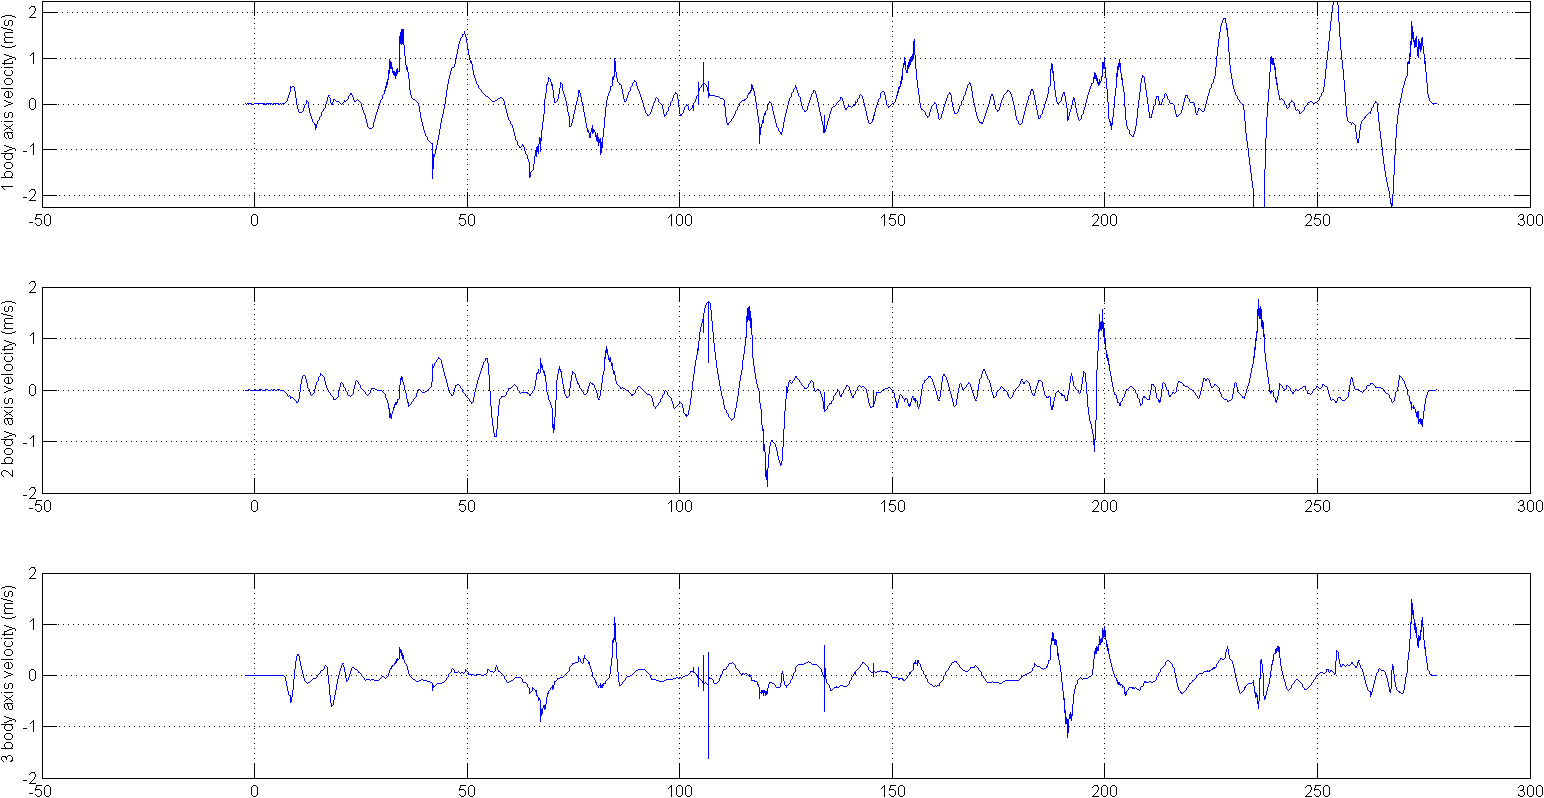
\includegraphics[width=\textwidth]{vel_sample.png}
\caption{Sample velocity time histories from characterization flight.}
\label{fig:vel_sample}
\end{figure}

Fig. \ref{fig:phi_align} shows time histories of the onboard estimated bank angle and the motion capture measurement. These histories were used to align the two clocks. A starting value of -2.57 seconds was used, and a value of -2.65 seconds was numerically solved for the time shift applied to the inertial clock.

\begin{figure}[tb!]
\centering
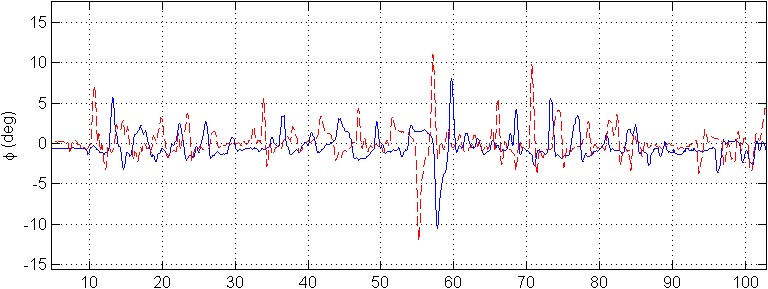
\includegraphics[width=0.7\textwidth]{phi_alignment.png}
\caption{Sample roll angle estimates and inertial measurements (blue) before time alignment.}
\label{fig:phi_align}
\end{figure}

Fig. \ref{fig:acc_opti_sample} shows accelerometer measurements, and motion capture equivalents after the $-g\U{n}_3$ value detected by the accelerometers is added to the motion capture accelerations in the body frame. There are clear regions where the Optitrack data are not usable due to large spikes from repeated numerical differentiation. There are many usable segments in which both data sources may be compared; e.g. $102.5 \leq t \leq 113.9$.

\begin{figure}[tb!]
\centering
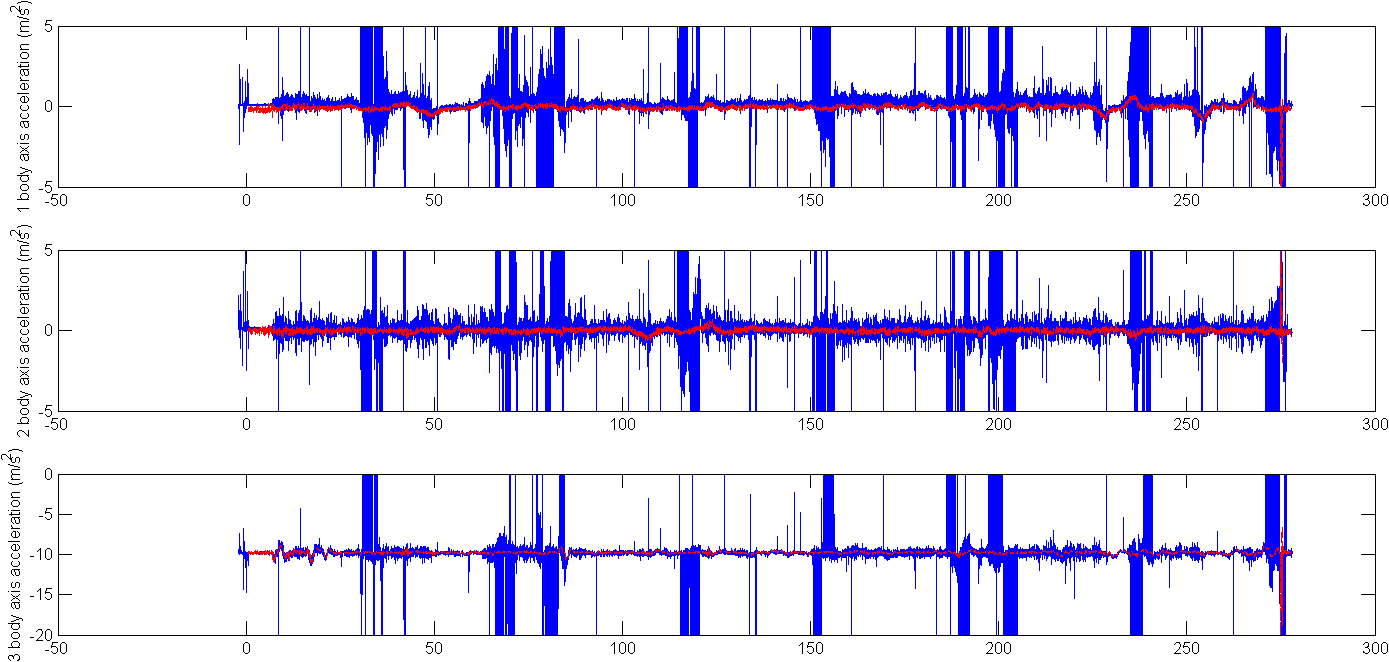
\includegraphics[width=\textwidth]{acc_opti_sample.png}
\caption{Sample accelerometer measurements and inertial equivalents (blue). Inertial values include the $-g$ term measured by the acclerometer.}
\label{fig:acc_opti_sample}
\end{figure}

\begin{table}[tb!]
\centering
\begin{tabular}{c|c|c}
Source & $\bar{\frac{\mu}{m}}$ & $S(\frac{\mu}{m})$ \\
\hline
Optitrack 1 & 0.1726 & 0.0703 \\
Accelerometer 1 & 0.2879 & 0.0310 \\
Optitrack 2 & 0.2704 & 0.0454 \\
\end{tabular}
\caption{Summary of model fitting results.}
\label{tab:modelResults}
\end{table}

Results are presented in terms of Optitrack-derived results from two days and accelerometer data from one day in Table \ref{tab:modelResults}. The motion capture- and accelerometer-based results from different days have similar mean and standard error. Since these data are from different sensors on different days, this value is assumed to be acceptably accurate. Taking a weighted average based on the number of flights in each day, the drag coefficient for the 3DR quadrotor is $0.28$. Without any further statistical analysis, we assume a normally distributed uncertainty with standard deviation $\sigma = 0.05$.

%\bibliography{references.bib}

\end{document}
